\documentclass[a4paper,10pt]{article}
\usepackage[utf8]{inputenc}
\usepackage{amsmath} 
\usepackage{xcolor}


\usepackage[cmtip,arrow]{xy}
\usepackage{pb-diagram,pb-xy}
\usepackage{graphics,amsfonts}
\usepackage{tikz}
\usepackage{authblk}
\usepackage{caption}
\usepackage{subcaption}


\usepackage{geometry}
 \geometry{
 a4paper,
 total={170mm,257mm},
 left=25mm,
 top=30mm,
 bottom=30mm,
 }


\baselineskip=0.30in
\textwidth=16cm
\textheight=24cm
\newcounter{theorem}

%TODO: send it to MATCH Communications in Mathematical and in Computer Chemistry
%exceptionally, on the top of the first page there must be 6 cm free space;
%tables and figures together with their captions (typed single spaced) must be inserted in the text;
%the pages must not be numbered;
%if possible (but not obligatorily) the number of pages should be even;

% \newcounter{defintion}[section]
% \newenvironment{definition}[1][]{\refstepcounter{definition}\par\medskip
%    \noindent \textbf{Definition~\theexample. #1} \rmfamily}{\medskip}

\newtheorem{definition}{Definition}[section]
\newtheorem{theorem}{Theorem}[section]
\newtheorem{problem}{Problem}[section]
\newtheorem{lemma}{Lemma}[theorem]
\newtheorem{proposition}{Proposition}[theorem]
\newtheorem{conjecture}[theorem]{Conjecture}
\newtheorem{observation}[theorem]{Observation}
\newtheorem{question}[theorem]{Question}
\newtheorem{remark}[theorem]{Remark}

\newtheorem{answer}[theorem]{Answer}
\newtheorem{warning}[theorem]{Warning!!!}

\newenvironment{proof}{\medskip\emph{Proof.}}{\hfill$\Box$\medskip}


\newcommand{\norml}{\vartriangleleft}

\newcommand{\Al}{{\rm Al}}
\newcommand{\Pl}{{\rm Pl}}

\DeclareMathOperator*{\supp}{supp}
\newcommand{\ZZ}{\mathbb{Z}}
\newcommand{\CC}{\mathbb{C}}
\newcommand{\DD}{\mathbb{D}}
\newcommand{\RR}{\mathbb{R}}
\newcommand{\C}{\mathcal{C}}
\newcommand{\B}{\mathcal{B}}
\newcommand{\F}{\mathcal{F}}
\newcommand{\R}{\mathcal{R}}
\newcommand{\G}{\mathcal{G}}
\renewcommand{\S}{\mathcal{S}}
\newcommand{\tG}{\tilde{G}}
\newcommand{\tg}{\tilde{g}}
\newcommand{\tGa}{\tilde{\Gamma}}
\newcommand{\Aut}{{\rm Aut}}
\newcommand{\Sym}{{\rm Sym}}
\newcommand{\Ker}{{\rm Ker}}
\newcommand{\Pet}{{\rm Pet}}
\newcommand{\PSL}{{\rm PSL}}
\newcommand{\AGL}{{\rm AGL}}
\newcommand{\core}{{\rm core}}
\newcommand{\razmak}{\hskip5mm}
\newcommand{\id}{{\rm id}}
\newcommand{\val}{{\rm val}}
\newcommand{\la}{\langle}
\newcommand{\ra}{\rangle}

\newcommand{\vGa}{\vec{\Gamma}}
\newcommand{\vDelta}{\vec{\Delta}}
\newcommand{\vW}{\vec{W}}

\newcommand{\LD}{\langle}
\newcommand{\RD}{\rangle}

\newcommand\TODO[1]{\textcolor{red}{#1}}
\newcommand\Tomo[1]{\textcolor{brown}{Tomo: #1}}
\newcommand\Nino[1]{\textcolor{green}{Nino: #1}}
\newcommand\Nancy[1]{\textcolor{Nancy: violet}{#1}}
\newcommand\Sarah[1]{\textcolor{Sarah: cyan}{#1}}
\newcommand\Jorg[1]{\textcolor{J\"{o}rg: blue}{#1}}
\newcommand\Thomas[1]{\textcolor{Thomas: orange}{#1}}
\newcommand\Patrick[1]{\textcolor{red}{Patrick: #1}}


%opening
\title{Convexity Numbers of Benzenoids}

\author[1,2]{Nino Ba\v{s}i\'{c}}
\author[3,4]{Sarah Berkemer}
\author[3]{J\"{o}rg Fallmann}
\author[5]{Patrick W. Fowler}
\author[3]{Thomas Gatter}
\author[1,2]{Toma\v{z} Pisanski}
\author[3,4]{Nancy Retzlaff}
\author[3,4]{Peter F. Stadler}
\affil[1]{University of Primorska, Koper, Slovenia}
\affil[2]{Institute of Mathematics, Physics and Mechanics, Ljubljana, Slovenia}
\affil[3]{Bioinformatics Group, Department for Computer Science, Leipzig University, Germany}
\affil[4]{Max-Planck-Institute for Mathematics in the Sciences, Leipzig, Germany}
\affil[5]{Department of Chemistry, University of Sheffield, Sheffield S3 7HF, UK}



\begin{document}
%\nocite{}

\maketitle

\begin{abstract}


In 2012, an important family of benzenoids was introduced by Cruz, Gutman and Rada which they
called convex benzenoids. In this paper we introduce a family of benzenoids that
resembles in many aspects to convex benezenoids and thus will be called pseudo-convex
benzenoids. Another family that contains both convex and pseudo-convex benzenoids called 
quasi-convex benzenoids is further introduced. 

A quasi-convex benzenoid is characterized by the fact that the average value of two consecutive 
numbers in its boundary code is never less than $2$. As a generalization of this approach we 
furthermore define a topological index for benzenoids that is called the convexity number. Finally, 
we investigate convexity numbers of several important families of benzenoids.
\end{abstract}

\textbf{Keywords:} benzenoid, convex benzenoid, pseudo-convex benzenoid, quasi-convex benzenoid.

%\section{Hexagonal grid}

%\begin{center}
%\begin{figure}
% 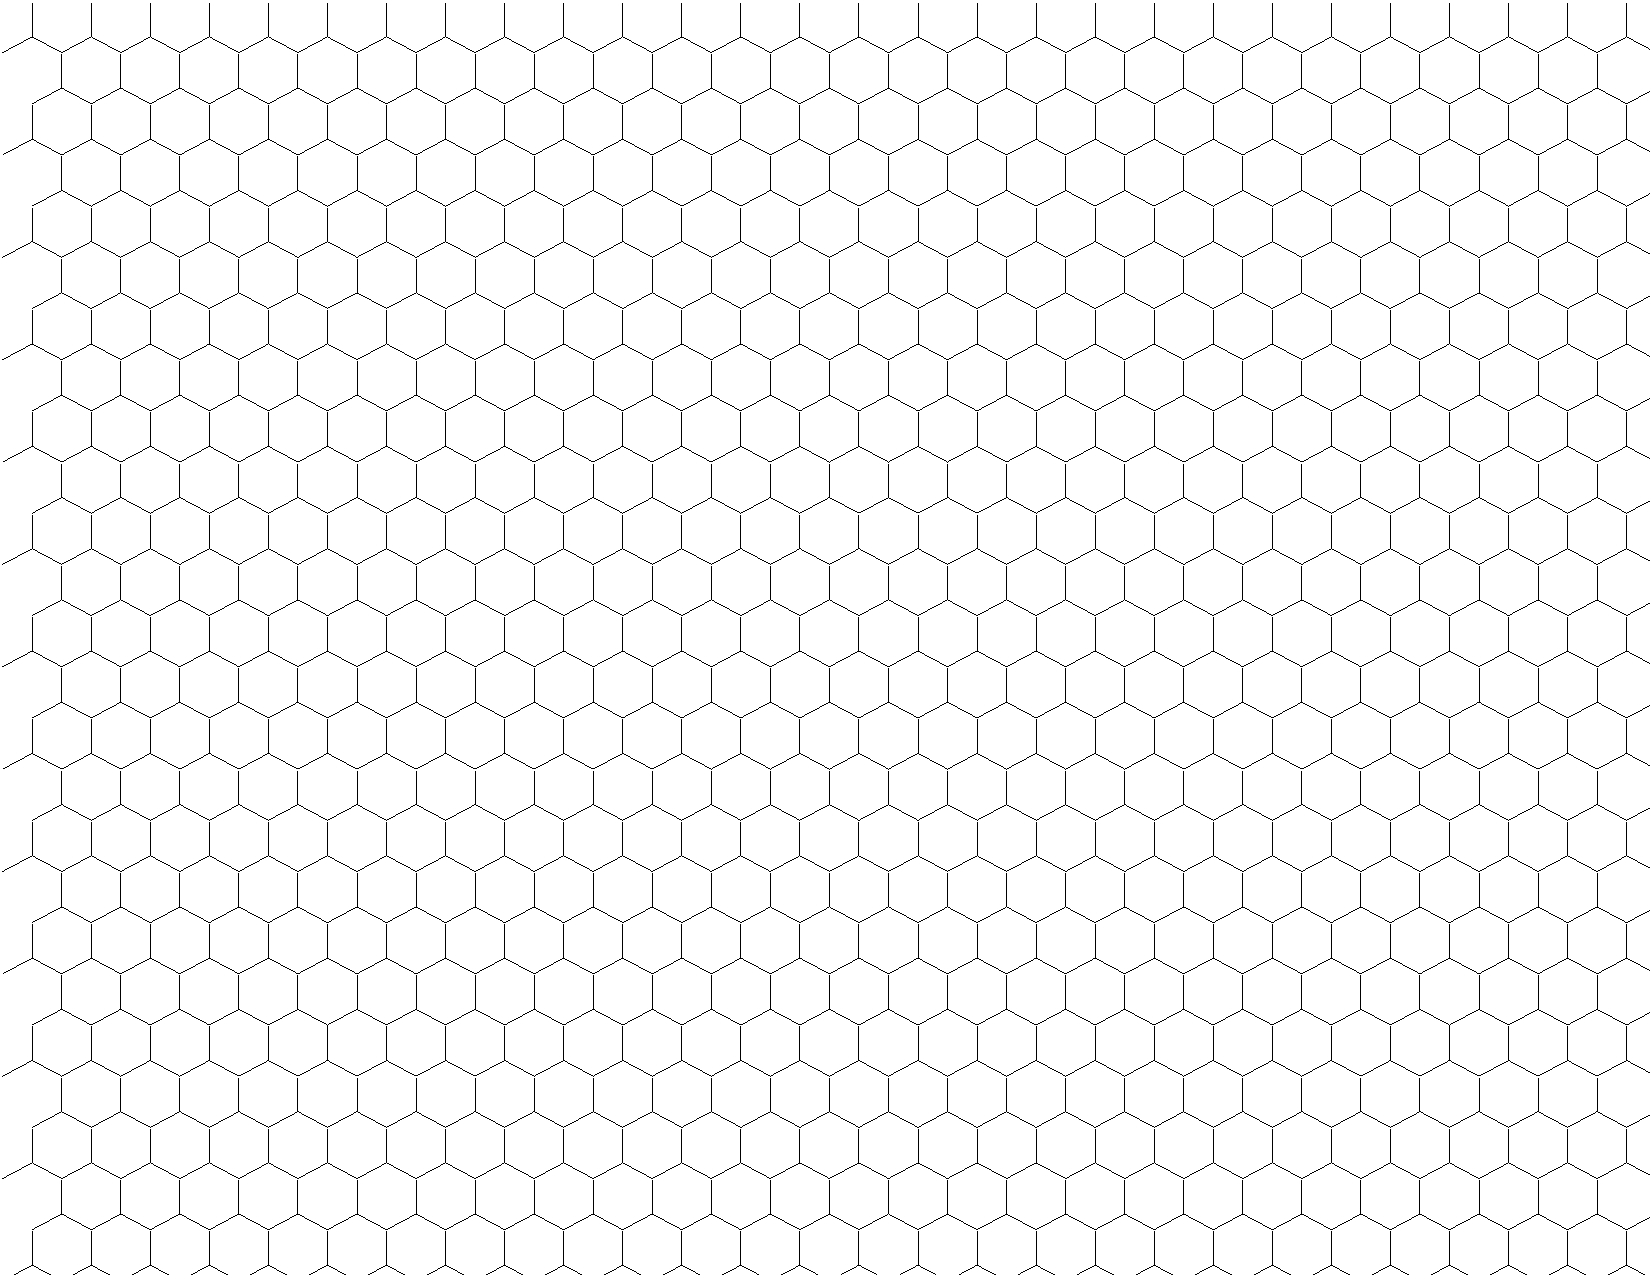
\includegraphics[width = 5cm,angle=180]{figures/hex.pdf}\\
%\label{fig:hex}
%\caption{$\bullet$ Benzenoid $B$ is a simply connected subgraph of the infinite hexagonal grid that is composed 
%of hexagons of the grid.%\footnote{Check correct definition elsewhere!}
%$\bullet$ Simply connected $\rightarrow$ no holes!
%$\bullet$ Beware of helicenes and coronenes!}
%\end{figure}
%\end{center}


\section{Introduction}

\emph{Benzenoids} form an important family of graphs. The reader is referred to the books \cite{cyvin_1988,gutman1989}. Each benzenoid can be uniquely described by 
a \emph{boundary-edges code} \cite{hansen1996}, a special sequence of numbers counting the number 
of edges between two vertices of valence 3, following the perimeter counter-clockwise. 
Benzene is an exception and is sometimes not
considered as a benzenoid. Figures \ref{fig3} and \ref{fig1} depict examples of benzenoid systems together with corresponding numbers in boundary-edges codes.

\Tomo{Make sure we define catacondensed and pericondensed benzenoids.}

\begin{figure}
\centering
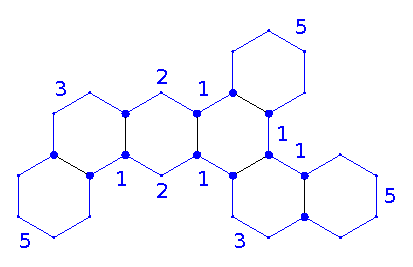
\includegraphics{figures/fig3}
\label{fig3}
\caption{A catacondensed benzenoid with boundary-edges code {\tt 532151153121} composed of 7 hexagons.}
\end{figure}


%\end{figure}

% \centering
\begin{figure}
\centering
 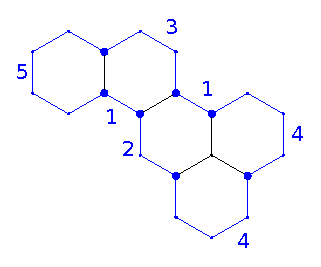
\includegraphics{figures/fig1}
 \label{fig1}\quad
 \caption{ A pericondensed benzenoid with boundary-edges code {\tt 5314421}, composed of of 5 hexagons. } 
\end{figure}


Recently, a special subfamily of \emph{convex benzenoids} has been introduced by Cruz, Gutman and Rada in \cite{CruGutRad12})
and enumerated by in \cite{basic2017}.

\begin{definition}
\label{def:original}
A benzenoid system $B$ is \emph{convex} if for any pair of its hexagons $a$ and $b$ the whole interval $I_\mathcal{H}(a,b)$ is contained in $B$.
\end{definition}

The main purpose of this paper is to investigate various generalizations of convexity.

\section{Boundary edges code revisited}

\begin{definition}
Let $c$ be a code. By $len(c)$ we denote the length of the code, ie. the number of symbols appearing in it, let $sum(c)$ denote the sum of all numbers of the code and let $con(c)$ we donote its \emph{contents}, that is incresing sequence of numbers appearing in $c$.
\end{definition}
For instance len({\tt 5314421}) = 7, sum({\tt 5314421}) = 20, con({{\tt 5314421}) = {\tt 12345}

Next we introduce the winding of a code.
\begin{definition}
Let $c$ be a code. By $w(c)$ we denote the winding of the code, where $w(c) = sum(c)-2len(c)$.
\end{definition}

\begin{lemma}
The winding of a concatenation of two (partial) codes $c$  and $d$ is additive: $w(c+d) = w(c)+w(d)$. 
\end{lemma}

\begin{lemma}
The winding of a valid benzenoid code $c$ is equal to $w(c) = 6$. 
\end{lemma}



\section{Isometric benzenoids}

In a convex benzenoid $B$ we require that all shortest paths between any two hexagons belong to $B$. If we relax the condition and require that at least one shortest path belongs to $B$ .

\begin{definition}
\label{def:isometric}
A benzeniod is isometric if the distances within benzenoid are the same as in the hexagonal grid.
%\Tomo{Explore this idea! See below! If the paper is too long we will leave it out for later.} 
\end{definition}



\begin{figure}
\centering
 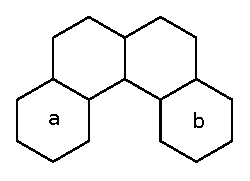
\includegraphics{figures/fig2}
 \label{fig2}
 \caption{Benzo[c]phenanthrene, $d_B(a, b) = 3 \neq d_{\mathcal{H}}(a, b) = 2$. This benzenoid is not isometric.}
\end{figure}

\begin{theorem}
Each convex benzenoid $B$ is isometric.
\end{theorem}
\begin{proof}
Take any shortest path $p$ between two hexagons $a$ and $b$ a convex benzenoid $B$. Since $B$ contains the whole interval between $a$ and $b$ the distance in $B$
between $a$ and $b$ is the same as the distance in the hexagonal grid. Hence $B$ must be isometric.
\end{proof}

In \cite{basic2017} one can find among other things the following results. Convex benzenoids admit boundaries in 6 directions.  Each convex benzenoid is obtained from an equilateral triangle by truncating some of its vertices. There exist 6 convex half-planes. Each of them has the code {\tt \ldots 2222222 \ldots}. In \cite{basic2017a} infinite convex benzenoids were studied. We will use and generalize the following characterization of convex benzenoids.

\begin{theorem}
A benzenoid is \emph{convex} if and only if it has no{ \tt 1} in its boundary edges code.
\end{theorem}

\section{$k$-convex benzenoids and convexity number.}
\begin{definition}
A benzenoid $B$ with boundary-edges code $c$ is $k$-convex if $k$ is the minimum value, such that the average of $k$ consecutive values in $c$ is always at least $2$. In this case $k$ is called \emph{convexity number} of $B$ and is denoted by $conv(B)$.
\end{definition}

Note that convexity number generalizes the notion of convexity for benzenoids.

\begin{theorem}
A benzenoid $B$ is $1$-convex ($conv(B) = 1$) if and only if $B$ is convex.
\end{theorem}

\begin{proof}
The average in this case is just the value itself and the result follows.
\end{proof}

%Before we state and prove the following result we will explore a bit more the boundary edges code.



\begin{theorem}
Any finite benzenoid $B$ is $k$-convex for some finite value of $k$.
\end{theorem}

\begin{proof}
Recall the definition of winding. Since $w(c) = sum(c)-2len(c) = 6$, we have $sum(c)/len(c) = 2 + 6/len(c) > 2$. Hence any finite benzenoid is $k$-convex at least for $k = len(c)$. 
\end{proof}



\begin{theorem}
There exist infinite benzenoids $B$ that are not $k$-convex for any finite value of $k$.
\end{theorem}

\begin{proof}
Here is an example: $\ldots 222212222 \ldots$.
\end{proof}

\begin{definition}
For any benzenoid $B$ let its \emph{convexity number} $conv(B)$ be $k$ if $B$ is $k$-convex. For infinite $B$, we may have $conv(B) = \infty$.
\end{definition}

\section{Quasi-convex and pseudo-convex benzenoids}

\begin{definition}
A $2$-convex benzenoid is called \emph{quasi-convex.}
\end{definition}


\begin{theorem}
A benzenoid is quasi-convex if and only if its boundary-edges code contains at least one {\tt 1} but no subsequence {\tt 11,12,21}.
\end{theorem}

\begin{proof}
A $2$-convex benzenoid is not convex, hence its code contains a 1. Let {\tt a,b} be two cyclicly consecutive numbers in its code. Since it is $2$-convex $a+b \geq 4$, hence {\tt 11},{\tt 12}{\tt 21} are
forbidden.  The converse also follows.  
\end{proof}


\begin{definition}
A benzenoid whose boundary-edges code contains at least one {\tt 1} but no subsequence {\tt 11,2} is called \emph{pseudoconvex}.
%\Tomo{New!}
\end{definition}

\begin{theorem}
Every pseudo-convex benzenoid is quasi-convex  but the converse is not true.
\end{theorem}

\begin{proof}
Follows readily.
\end{proof}


\begin{theorem}
Every quasi-convex benzenoid is isometric but the converse is not true.
\end{theorem}
\begin{proof}
It is easy to find an isometric benzenoid that is not quasi-convex. Actually, one can construct a sequence of isometric benzenoids with
increasing convexity numbers.

The implication is more involved.
\Tomo{Needs to be completed!}


\end{proof}


\section{Half-planes}

For us, a (benzenoid) half-plane is a benzenoid that contains all hexagons that have a non-empy intersection with an Euclidean half-plane. 

Clearly, there are 6 convex half-planes, all described by the same two-way infinite boundary edges code: {\tt \ldots 222222 \ldots}. 
There exist 6 pseudoconvex half-planes. {\tt \ldots 131313131313 \ldots}. It is interesting that no other quasi-convex half-planes exist.

\begin{theorem}
Every quasi-convex half plane is pseudo-convex.
\end{theorem}
\begin{proof}
Let us assume that there exists a half-plane $H$ that is quasi-convex. In particular it means that $con(H)$ contains no {\tt 4,5,6}. Since $H$ is a half-plane it must have a straight boundary: $w(H) = 0$.  In particular it means there are three cases for $con(H)$:

$\bullet$ $con(H) = 2$

$\bullet$ $con(H) = 13$

$\bullet$ $con(H) = 123$

Note that the other possiblities, such as $con(H) = 12$ are ruled out since they ar unbalenced and would never produce $w(H) = 0$.


Case $con(H) = 2$ gives rise exactly to convex half-planes.

Consider now $con(H) = 13$. It is not hard to see that if $H \neq {\tt \ldots 131313131313 \ldots}$ then there must be at least two consecutive values of 3 present in the code. However, since no two consecutive values of 1 are allowed in a quasi-convex case, that would imply $w(H) \neq 0$, a contradiction.

Finally let $con(H) = 123$. If we have a sequence of 2s that is not infinite in both directions, the last 2 in the sequence must be followed by a 3. This, in turn, cannot be followed either by 2 or 3. So we must have a local picture ${\tt \ldots 22231}$. This implies teh rest of the sequence 
${\tt \ldots 22231313131 \ldots}$. Unfortunately such a sequence is bent
and cannot be continued to form a quasi-convex $H$ with $w(H) = 0$.

 
\end{proof}



\begin{theorem}
A benzenoid is convex if and only if it is an intersection of $h$ convex halfplanes. At most 6 of them
are needed.
\end{theorem}

\begin{theorem}
A benzenoid is pseudo convex if and only if it is an intersection of $h$ pseudo convex halfplanes. At most 6 of them are needed.
\end{theorem}

\begin{theorem}
A benzenoid is quasi convex if and only if it is an intersection of $h$ convex or pseudo convex halfplanes. 
At most 12 of them are needed and one of them must be pseudo convex.
\end{theorem}


\section{Analysis of small benzenoids and benzenoid families}

In this section we give basic statistics of benzenoids.


\begin{figure}
\centering
 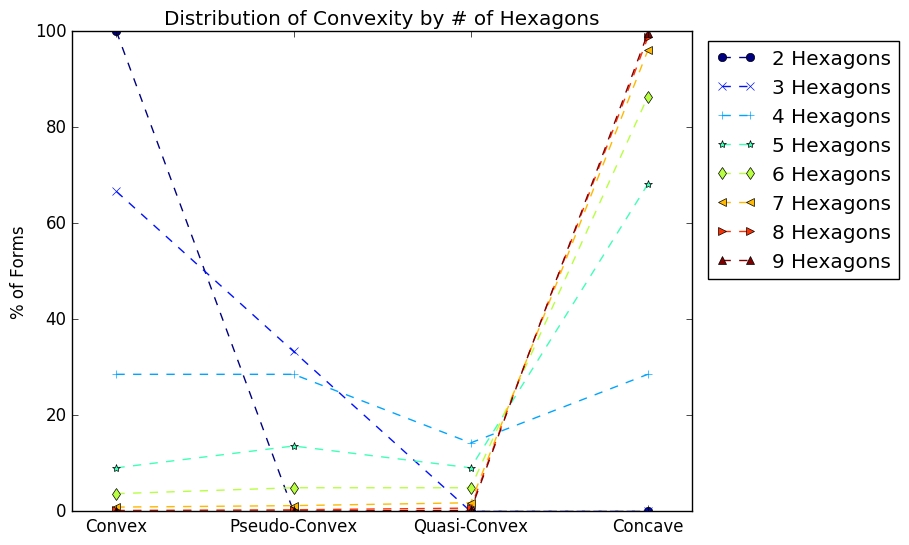
\includegraphics[width=100mm]{figures/distribution_of_convexity.png}
 \label{fig_convex}
 \caption{Distribution of kinds of convexity for benzoids of different length. For larger benzoids most structures are not convex}
\end{figure}

\begin{figure}
\centering
 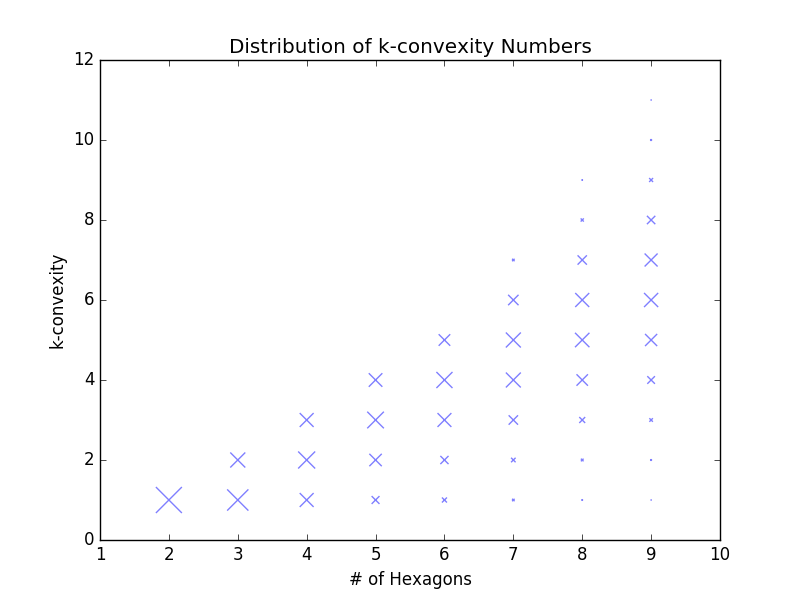
\includegraphics[width=100mm]{figures/distribution_of_k_values}
 \label{fig_k}
 \caption{Distribution of k-convexity for benzoids of different sizes. Marker size indicates abundance of forms with this k-convexity. The size of markers are corrected by abundance for each column (for each number of hexagons in the benzoid}
\end{figure}

\begin{table}
 \caption{Overview of the smallest benzoids for each $k$-convexity. Number of hexagons, number of benzoids with same length and $k$ and an example boundary code are given.}
 \medskip
 \begin{tabular}{|l l l l|}
 \hline
  $k$-convexity number & \# Hexagons & \# Benzoids & example boundary code \\
  \hline
  1 & 2 & 1 & 55 \\
  2 & 3 & 1 & 5351 \\
  3 & 4 & 2 & 532521 \\
  4 & 5 & 6 & 52325212\\
  5 & 6 & 16 & 5232252212\\
  6 & 7 & 53 & 51513244111\\
  7 & 7 & 3 & 523315151112\\
  8 & 8 & 21 & 52151315151112\\
  9 & 8 & 2 & 53323325211211\\
  10 & 9 & 23 & 5223315125211122\\
  11 & 9 & 3 & 5332332252211211\\
  \hline
 \end{tabular}
\end{table}
\begin{problem}
Identify all families of quasi-convex and pseudo-convex benzenoids.
\end{problem}


\begin{problem}
Enumerate all quasi-convex (pseudo-convex) benzenoids.
\end{problem}


\begin{problem}
Identify all families of isometric benzenoids.
\end{problem}

\begin{problem}
Enumerate all isometric benzenoids.
\end{problem}

\begin{problem}
Among all convex/quasi convex/pseudo convex benzenoids on $n$ hexagons identify the ones with extreme values of a given topological index.
\end{problem}

\begin{problem}
Among all benzenoids on $n$ hexagons identify the ones with extreme values of convexity number..
\end{problem}

One may ask a practical question concerning convexity number of benzenoids

\begin{problem}
Explore the relationship between convexity number of existing benzenoids and there physical and chemical properties.
\end{problem}

Convexity number does not tell us anything about the distribution of average consecutive numbers of the boundary edges code.
Let $c(B) = [c_0,c_1,\ldots, c_{m-1}]$ be the boundary edges code of benzenoid $B$. The indices $i$ in $c_i$ are considered mod $m$. 

\begin{definition}
Let $a(c(B),i,k)$ and $A(c(B),k)$ be defined as follows:
$$a(c(B),i,k) = (c_i + c_{i+1}+c_{i+2}+\ldots+c_{i+k-1})/k$$ 
$$A(c(B),k) = \min_{i =0}^{m-1}a(c(B),i,k)$$
\end{definition}


\begin{theorem}
For every $k$ we have $1\leq A(c(B),k) \leq A(c(b),k+1) \leq 3$\footnote{not sure about the upper bound}
\end{theorem}


\begin{problem}
Study the distribution of $a(c(B),i,k)$ for small values of $k$ (up to the convexity number of $B$. Compare the minimum with the average and maximum.
\end{problem}



%\begin{center}
%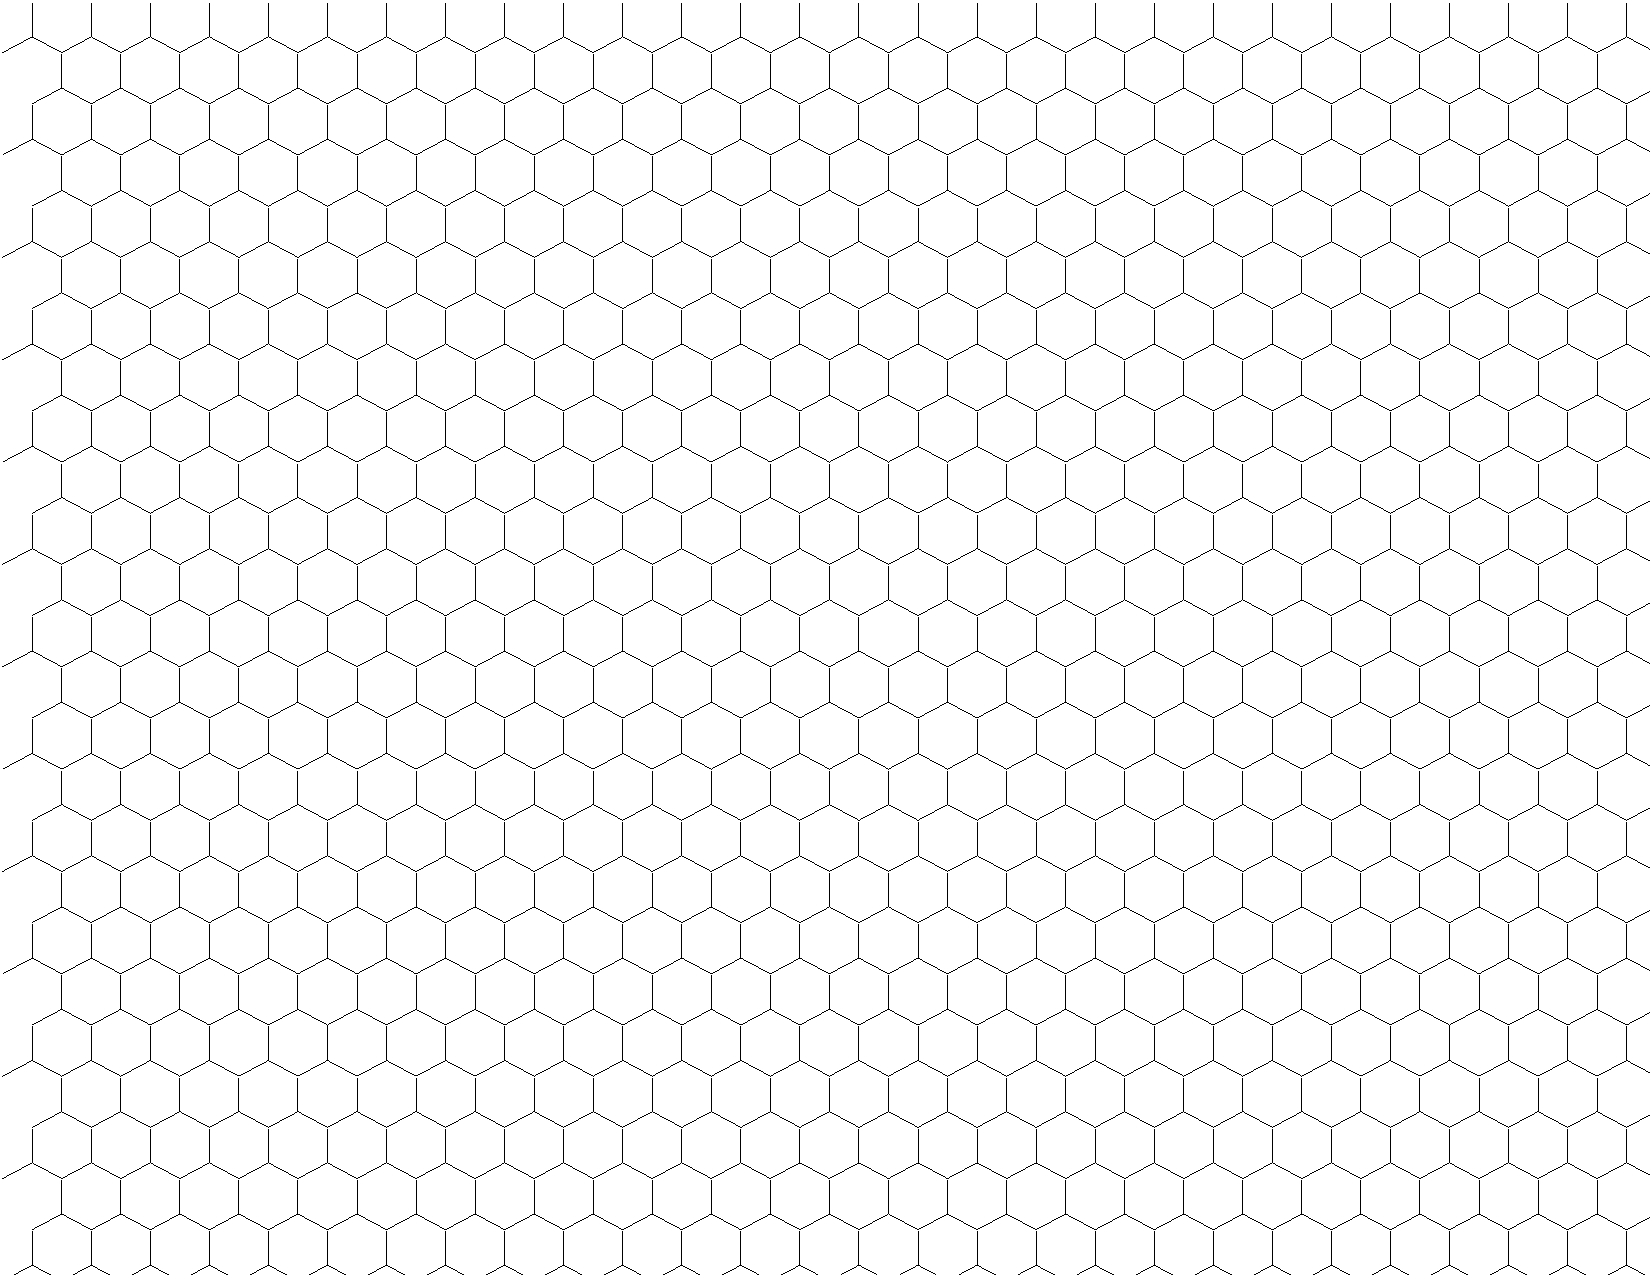
\includegraphics[width = 10cm,angle=180]{figures/hex.pdf}\\
%\medskip
%\end{center}
\section{The contents of the boundary edges code}
\Tomo{Should this be a separate paper?}

In general we have $2^6-1 = 63$ cases. We would like to identify the ones that are
\begin{enumerate}
\item impossible
\item have finite number of finite realization
\end{enumerate}

\begin{enumerate}
\item $con(B) = {\tt 1}$ impossible
\item $con(B) = {\tt 2}$ convex halfplane
\item $con(B) = {\tt 3}$ only one finite case: {\tt 333333}
\item $con(B) = {\tt 4}$ only one finite case:{\tt 444}
\item $con(B) = {\tt 5}$ only one finite case:{\tt 55}
\item $con(B) = {\tt 6}$ only one finite case: {\tt 6}
\item $con(B) = {\tt 12}$ no finite cases. Here {\tt 1} appears at most 3 times.
\item No other case involving {\tt 6} is possible.
\item All other cases are realisable by countably many finite and uncountably 
many infinite benzenoids
\end{enumerate}


\section{Some Generalizations on Boundary Codes for known Benzenoid Families}

\subsection{Catacondensed Single Chains with one, two or three Segments}

Cyvin and Gutman~\cite[p.~62]{cyvin_1988} 

\subsubsection{One Segment}
single chains:

$L(n) = 52^{n-2}52^{n-2} , n>1$

\subsubsection{Two Segments}

$M2(m,n) = 52^{m-2}12^{n-2}52^{n-2}32^{m-2}, m,n>1$

\subsubsection{Three Segments}

1) $M3(m,n,k) = 52^{k-2}12^{m-2}12^{n-2}52^{n-2}32^{m-2}32^{k-2}, m,n,k>1$


2) $Z3(m,n,k) = 52^{n-2}12^{k-2}32^{m-2}52^{m-2}12^{k-2}32^{n-2} m,n,k>1$


\subsection{Catacondensed Single Zigzag Chain}

Cyvin and Gutman~\cite[p.~63]{cyvin_1988}

\cite{gordon_1952}
\cite{yen_1971}
\cite{balaban_1985}

$n = 1 : W(\mu,1) = 6$\\
$n > 1 : W(\mu,n) =5 2^{\mu-2} (3 2^{\mu-2} 1 2^{\mu-2})^{\lfloor\frac{n-2}{2}\rfloor} (3 2^{\mu-2})^{n \mod 2}
5 2^{\mu-2} (1 2^{\mu-2}3 2^{\mu-2})^{\lfloor\frac{n-2}{2}\rfloor} (1 2^{\mu-2})^{n \mod 2}$

\begin{table}4
 \caption{Overview for smaller Catacondensed Single Zigzag Chains: variables $m$, $n$, their specific boundary code and calculated $k$-convexity number}
 \medskip
 \begin{tabular}{|l l l r|}
  \hline
  $\mu$ & $n$ & boundary code & $k$-convexity number\\
  \hline
  (2 & 2 & 5252 & 1)\\
  2 & 3 & 52325212 & 4\\
  3 & 3 & 522322522122 & 6\\
  4 & 3 & 5222322252221222 & 8\\
  \hline
  2 & 4 & 523212521232 & 4\\
  3 & 4 & 522322122522122322 & 6\\
  4 & 4 & 522232221222522212223222 & 8\\ 
  \hline
 \end{tabular}
\end{table}

$conv(W(\mu,n)) = 2*(\mu-1)+2$ since $\mu-1$ is the length of one $2$-chain before 
and as well as after $1$.


\subsection{Chevron}
Cyvin and Gutman~\cite[p.~111]{cyvin_1988}


\cite{gordon_1952}
\cite{cyvin_1985}

$n = 1, k,m > 1 : 5 2^{k-2} 3 2^{m-2} 5 2^{m-2} 1 2^{k-2}$\\
$k,m,n > 1 : 4 2^{n-2} 3 2^{k-2} 3 2^{m-2} 3 2^{n-2} 4 2^{m-2} 1 2^{k-2}$

\begin{table}
 \caption{Overview for smaller Chevrons: variables $k$, $m$, $n$, their specific boundary code and calculated $k$-convexity number}
 \medskip
 \begin{tabular}{|l l l l r|}
 \hline
  $k$ & $m$ & $n$ & boundary code & $k$-convexity number\\
  \hline
  2 & 2 & 1 & 5351 & 2\\
  \hline
  3 & 2 & 1 & 523512 & 3\\
  4 & 2 & 1 & 52235122 & 4\\
  5 & 2 & 1 & 5222351222 & 5\\
  \hline
  2 & 3 & 1 & 532521 & 3\\
  2 & 4 & 1 & 53225221 & 4\\
  2 & 5 & 1 & 5322252221 & 5\\
  \hline
  2 & 2 & 2 & 433341 & 2\\
  2 & 3 & 2 & 43323421 & 3\\
  2 & 4 & 2 & 4332234221 & 4\\
  2 & 5 & 2 & 43322234221 & 5\\
  \hline 
  2 & 2 & 3 & 42333241 & 2\\
  2 & 2 & 4 & 4223332241 & 2\\
  2 & 2 & 5 & 422233322241 & 2\\
  \hline
  3 & 2 & 2 & 43233412 & 3\\
  4 & 2 & 2 & 4322334122 & 4\\
  5 & 2 & 2 & 432223341222 & 5\\
  \hline
  3 & 3 & 3 & 423232324212 & 4\\
  3 & 4 & 3 & 42323223242212 & 5\\
  3 & 5 & 3 & 4232322232422212 & 6\\
  \hline
 \end{tabular}
\end{table}

$k-convexity = 2 + (m-2) + (k-2)$ where $(m-2)$ and $(k-2)$ are depicting the 
length of $2$-chains surrounding $1$. Hence $1$ and another edge code has to be
counted.

\subsection{Multiple Zigzag Chain}

Cyvin and Gutman~\cite[p.~143]{cyvin_1988}

\cite{gordon_1952}
\cite{cyvin_1986}
\cite{cyvin_1985}
\cite{cyvin_1986number}
\cite{gutman_1987}

$A(1,1) = 6$\\
$A(1,2) = A(2,1) =55$\\
$A(2,2) = 4343$\\
$A(m,2) = 5 (31)^{\lfloor\frac{m-2}{2} \rfloor} 3^{m \mod 2} 5 1^{m \mod 2}  (31)^{\lfloor\frac{m-2}{2} \rfloor}, m>2$\\
$A(m,n) = 4 2^{n-2} 3  (31)^{\lfloor\frac{m-2}{2} \rfloor}  3^{m \mod 2} 4 2^{n-2} 3  1^{m \mod 2}  (31)^{\lfloor\frac{m-2}{2} \rfloor}, m,n>2$

\begin{table}
 \caption{Overview for smaller Multiple Zigzag Chains: variables $m$, $n$, their specific boundary code and calculated $k$-convexity number}
 \medskip
 \begin{tabular}{|l l l r|}
 \hline
  $m$ & $n$ & boundary code & $k$-convexity number\\
  \hline
  (2 & 2 & 4343 & 1) \\
  3 & 2 & 5351 & 2 \\
  4 & 2 & 531531 & 2 \\
  5 & 2 & 53135131 & 2 \\
  3 & 2 & 5351 & 2 \\
  3 & 3 & 42334231 &  \\
  3 & 4 & 4223342231 & 2 \\
  3 & 5 & 422233422231 & 2 \\
  4 & 2 & 531531 & 2 \\
  4 & 3 & 4233142331 & 2 \\
  4 & 4 & 422331422331 & 2 \\
  4 & 5 & 42223314222331 & 2 \\
  \hline
 \end{tabular}
\end{table}

The $k$-convexity number is $2$ since there is no $1$ followed by $2$.

\begin{figure}
 \centering
 \begin{subfigure}{0.275\textwidth}
  \centering
  %\includegraphics[0.25\textwidth]{}
  \caption{}
  \label{fig:}
 \end{subfigure}
 \begin{subfigure}{0.275\textwidth}
  \centering
  %\includegraphics[0.25\textwidth]{}
  \caption{}
  \label{fig:}
 \end{subfigure}
 \begin{subfigure}{0.43\textwidth}
  \centering
  %\includegraphics[0.415\textwidth]{}
  \caption{}
  \label{fig:}
 \end{subfigure}
 \caption{blubb}
\end{figure}



\subsection{Prolate Pentagon}

Cyvin and Gutman~\cite[p.~182]{cyvin_1988}

\cite{cyvin_1987}


$A(1,1) = 6$\\
$A(1,n) = 52^{n-2}52^{n-2}, n>1$\\
$A(m, 1) = 51(31)^{m-2}52^{m-2}32^{m-2}, m>1$\\
$A(m,n) = 32^{n-2}41(31)^{m-2}42^{n-2}32^{m-2}32^{m-2}, m,n>1$

\begin{table}
 \caption{Overview for smaller Prolate Pentagons: variables $m$, $n$, their specific boundary code and calculated $k$-convexity number}
 \medskip
 \begin{tabular}{|l l l r|}
 \hline
  $m$ & $n$ & boundary code & $k$-convexity number\\
  \hline
  2 & 1 & 515 & 2 \\
  3 & 1 & 5131523 & 2 \\
  4 & 1 & 51313152233 & 2 \\
  5 & 1 & 513131315222333 & 2 \\
  \hline
  2 & 2 & 341433 & 2 \\
  3 & 2 & 3413143232 & 2 \\
  4 & 2 & 34131314322322 & 2 \\
  5 & 2 & 341313131432223222 & 2 \\
  \hline
  2 & 3 & 32414233 & 2 \\
  3 & 3 & 324131423232 & 2 \\
  4 & 3 & 3241313142322322 & 2 \\
  5 & 3 & 32413131314232223222 & 2 \\
  \hline
  2 & 4 & 3224142233 & 2 \\
  3 & 4 & 32241314223232 & 2 \\
  4 & 4 & 322413131422322322 & 2 \\
  5 & 4 & 3224131313142232223222 & 2 \\
  \hline
 \end{tabular}
\end{table}

The $k$-convexity stays $2$ since there are $1$s but they are never followed by $2$
or less.


\subsection{Prolate Triangle}

Cyvin and Gutman~\cite[p.~197]{cyvin_1988}

\cite{cyvin_2013}


$A(m) = 51(31)^{m-2}52^{m-2}32^{m-2}, m>1$

\begin{table}
 \caption{Overview for smaller Prolate Triangle: variable $m$, the specific boundary code and calculated $k$-convexity number}
 \medskip
 \begin{tabular}{|l l r|}
 \hline
  $m$ & boundary code & $k$-convexity number\\
  \hline
  2 & 5153 & 2 \\
  3 & 51315232 & 2 \\
  4 & 513131522322 & 2 \\
  5 & 5131313152223222 & 2 \\
  6 & 51313131315222232222 & 2 \\
  \hline
 \end{tabular}
\end{table}


\subsection{Problate Triangle}

Cyvin and Gutman~\cite[p.~197]{cyvin_1988}


\cite{cyvin_2013}


$A(m) = 4(31)^{m-1} 52^{m-1}32^{m-2}, m>1$

\begin{table}
 \caption{Overview for smaller Problate Triangles: variable $m$, the specific boundary code and calculated $k$-convexity number}
 \medskip
 \begin{tabular}{|l l r|}
 \hline
  $m$ & boundary code & $k$-convexity number\\
  \hline
  2 & 43153 & 2 \\
  3 & 431315232 & 2 \\
  4 & 4313131522322 & 2 \\
  5 & 43131313152223222 & 2 \\
  6 & 431313131315222232222 & 2 \\
  \hline
 \end{tabular}
\end{table}

Same as above.

\subsection{Oblate Triangle}

Cyvin and Gutman~\cite[p.~197]{cyvin_1988}

\cite{cyvin_2013}


$A(m) = 43(13)^{m-2}42^{m-2}32^{m-2}, m>1$

\begin{table}
 \caption{Overview for smaller Oblate Triangles: variable $m$, the specific boundary code and calculated $k$-convexity number}
 \medskip
 \begin{tabular}{|l l r|}
 \hline
  $m$ & boundary code & $k$-convexity number\\
  \hline
  (2 & 55 & 1) \\
  3 & 43134232 & 2 \\
  4 & 431313422322 & 2 \\
  5 & 4313131342223222 & 2 \\
  6 & 43131313134222232222 & 2 \\
  \hline
 \end{tabular}
\end{table}


\subsection{Prolate Rectangle}

Cyvin and Gutman~\cite[p.~201]{cyvin_1988}


\cite{cyvin_2013}
\cite{yen_1971}

$A(m,n) = 42^{n-2}4(13)^{m-2}142^{n-2}4(13)^{m-2}1, m,n>1$

\begin{table}
 \caption{Overview for smaller Prolate Rectangle: variables $m$, $n$ their specific boundary code and calculated $k$-convexity number}
 \medskip
 \begin{tabular}{|l l l r|}
 \hline
  $m$ & $n$ & boundary code & $k$-convexity number\\
  \hline
  2 & 2 & 44144 & 2 \\
  3 & 2 & 441314413 & 2 \\
  4 & 2 & 4413131441313 & 2 \\
  5 & 2 & 44131313144131313 & 2 \\
  \hline
  3 & 2 & 441314413 & 2 \\
  3 & 3 & 42413142413 & 2 \\
  3 & 4 & 4224131422413 & 2 \\
  3 & 5 & 422241314222413 & 2 \\
  \hline
  4 & 2 & 4413131441313 & 2 \\
  4 & 3 & 424131314241313 & 2 \\
  4 & 4 & 42241313142241313 & 2 \\
  4 & 5 & 4222413131422241313 & 2 \\
  \hline
 \end{tabular}
\end{table}

See above


\subsection{Dihedral all-Benzenoids}

Cyvin and Gutman~\cite[p.~215]{cyvin_1988}

quasi convex

$s_m: A(m)_{s_m} 51215(13)^{m-1}151215(13)^{m-1}1, m>0$
\cite{zhang_1986}

\begin{table}
 \caption{Overview for smaller Dihedral all-Benzenoids $s_m$: variable $m$, the specific boundary code and calculated $k$-convexity number}
 \medskip
 \begin{tabular}{|l l r|}
 \hline
  $m$ & boundary code & $k$-convexity number\\
  \hline
  1 & 512151512151 & 4 \\
  2 & 5121513151215131 & 4 \\
  3 & 51215131315121513131 & 4 \\
  4 & 512151313131512151313131 & 4 \\
  5 & 5121513131313151215131313131 & 4 \\
  \hline
 \end{tabular}
\end{table}

The $k$-convexity is always $4$ since the smallest molcule already contains a chain 
$121$ which average is only bigger than $2$ when combined with a number greater than $3$.



$t_m: A(m)_{t_m} 41414(13)^{m-2}141414(13)^{m-2}1, m>1$

\cite{zhang_1986}


\begin{table}
 \caption{Overview for smaller Dihedral all-Benzenoids $t_m$: variable $m$, the specific boundary code and calculated $k$-convexity number}
 \medskip
 \begin{tabular}{|l l r|}
 \hline
  $m$ & boundary code & $k$-convexity number\\
  \hline
  2 & 414141414141 & 2 \\
  3 & 4141413141414131 & 2 \\
  4 & 41414131314141413131 & 2 \\
  5 & 414141313131414141313131 & 2 \\
  6 & 4141413131313141414131313131 & 2 \\
  \hline
 \end{tabular}
\end{table}

Always $2$ since the smallest number adjacent to $1$ is $3$.


\subsection{Some named benzenoids and some of their features.}


\begin{table}
 \caption{List of small benzenoids and their features. The list is complete up to 4 hexagons.}
\medskip 
\begin{tabular}{|llrlr|}
  \hline
  name & boundary code & \# hexagons & class & $k$-convexity number\\
  \hline
  Benzene & 6 & 1 & convex & 1\\
  \hline
  Naphthaline & 55 & 2 & convex & 1\\
  \hline
  Phenalene & 444 & 3 & convex & 1\\
  Anthracene & 5252 & 3 & convex & 1\\
  Phenanthrene & 5351 & 3 & pseudo-convex & 2\\
  \hline
  Tetracene & 522522 & 4 & convex & 1\\
  Pyrene & 4343 & 4 & convex & 1\\
  .. & 52441 & 4 & quasi-convex & 2\\
  Chrysene & 513513 & 4 & pseudo-convex & 2\\
  Triphenylene & 515151 & 4 & pseudo-convex & 2\\
  Benzo(c)phenanthrene & 533511 & 4 & ? & 3\\
  Benz(a)anthracene & 512523 & 4 & ?, & 3\\
  Benz(a)anthracene(2) & 521532 & 4 & ? & 3\\
  \hline
  Olympicene & 42433 & 5 & convex & 1\\
  Pentacene & 52225222 & 5 & convex & 1\\
  Picene & 51315313 & 5 & pseudo-convex & 2\\
  Helicene & 53335111 & 5 & ? & 2\\
  Perylene & 441441 & 5 & pseudo-convex & 2\\
  Benzo(a)pyrene & 513432 & 5 & quasi-convex & 2\\
  Benzo(e)pyrene & 514341 & 5 & pseudo-convex & 2\\
  Dibenz(a,h)anthracene & 53215321 & 5 & ? & 3\\
  Pentaphen & 52125232 & 5 & ? & 4\\
  Dibenz(a,j)anthracene & 51215323 & 5 & ? & 4\\
  \hline
  Anthanthrene & 324324 & 6 & convex & 1\\
  Hexacene & 5222252222 & 6 & convex & 1\\
  Benzo(ghi)perylene & 414333 & 6 & pseudo-convex & 2\\
  Zethrene & 42144214 & 6 & ? &3\\
  \hline
  Coronene & 333333 & 7 & convex & 1\\
  Heptacene & 522222522222 & 7 & convex & 1\\
  \hline
  Ovalene & 33323332 & 10 & convex & 1\\
  \hline
  Dicoronylene & 23333212333321 & 15 & ? & 4\\
  \hline
\end{tabular}
\end{table}

\section{Conclusion}



\section*{Acknowledgements}
\TODO{other Fundings?}\\
TG would like to thank the Deutsche Forschungsgemeinschaft (DFG STA 850/19-2 within SPP 1738).
All the authors thank the DAAD - PPP Slowenien "Mathematical Foundations of Selected 
Topics in Science".
 
%\nocite{*}

\bibliographystyle{abbrv}
\bibliography{benzenoids}

\end{document}
